
All high-performance computers today have multiple CPUs or multiple CPU cores (independent processors in a single package). Even most laptop computers have at least two, often four, cores. As we have said many times, in the context of performance, efficiency is not leaving any hardware idle; a program cannot be efficient or high-performing if it uses only a fraction of the computing power, such as one of many CPU cores. There is only one way for a program to use more than one processor at a time: we have to run multiple threads or processes. As a side note, this isn't the only way to use multiple processors for the benefit of the user: very few laptops, for example, are used for high-performance computing. Instead, they use multiple CPUs to better run different and independent programs at the same time. It is a perfectly good use model, just not the one we are interested in in the context of high-performance computing. HPC systems usually run one program on each computer at any time, even one program on many computers in case of distributed computations. How does one program use many CPUs? Usually, the program runs multiple threads.

\subsubsubsection{5.2.1\hspace{0.2cm}What is a thread?}

A thread is a sequence of instructions that can be executed independently of other threads. Multiple threads are running concurrently within the same program. All threads share the same memory, so, by definition, threads of the same process run on the same machine. We have mentioned that an HPC program can also consist of multiple processes. A distributed program runs on multiple machines and utilizes many separate processes. The subject of distributed computing is outside the scope of this book: we are learning how to maximize the performance of each of these processes.

So, what can we say about the performance of multiple threads? First of all, having multiple instruction sequences execute at the same time is beneficial only if the system has enough resources actually to execute them at the same time. Otherwise, the operating system is just switching between different threads to allow each one a time slice to execute.

On a single processor, a thread that is busy computing provides as much work as the processor can handle. This is true even if the thread is not using all of the computing units or is waiting on memory accesses: the processor can execute only one instruction sequence at a time – it has a single program counter. Now, if the thread is waiting on something, such as user input or network traffic, the CPU is idle and could execute another thread without impacting the performance of the first one. Again, the operating system handles the switching between the threads. Note that waiting on memory does not count as waiting in this sense: when a thread is waiting on memory, it just takes longer to execute one instruction. When a thread is waiting on I/O, it has to make an operating system call, then it's blocked by the OS and isn't executing anything at all until the OS wakes it up to process the data.

All threads that do heavy computing require adequate resources if the goal is to make the program more efficient overall. Usually, when we think about resources for threads, we have in mind multiple processors or processor cores. But there are other ways to increase resource utilization through concurrency as well, as we are about to see.

\subsubsubsection{5.2.2\hspace{0.2cm}Symmetric multi-threading}

We have mentioned several times throughout the book that a processor has a lot of computing hardware, and most programs rarely, if ever, use all of it: the data dependencies in the program limit how much computation the processor can do at any time. If the processor has spare computing units, can't it execute another thread at the same time to improve efficiency? This is the idea behind Symmetric Multi-Threading (SMT), also known as hyper-threading.

An SMT-capable processor has a single set of registers and computing units, but two (or more) program counters and an extra copy of whatever additional hardware it uses to maintain the state of a running thread (the exact implementation varies from one processor to another). The end result is: a single processor appears to the operating system and the program as two (usually) or more separate processors, each capable of running one thread. In reality, all threads running on one CPU compete for the shared internal esources such as registers. The SMT can offer significant performance gains if each thread does not make full use of these shared resources. In other words, it compensates for the inefficiency of one thread by running several such threads.

In practice, most SMT-capable processors can run two threads, and the performance gains vary widely. It is rare to see 100\% speedup (two threads both run at full speed). Usually, the practical speedup is between 25\% and 50\% (the second thread is effectively running at quarter-speed to half-speed), but some programs get no speedup at all. For the purposes of this book, we will not treat the SMT threads in any special way: to the program, an SMT processor appears as two processors, and anything we say about the performance of two real threads running on separate cores applies equally to the performance of two threads that happen to run on the same core. At the end of the day, you have to measure whether running more threads than you have physical cores provides any speedup to your program and, based on that, decide how many threads you want to run.

Whether we're sharing entire physical cores or the logical cores created by the SMT hardware, the performance of a concurrent program largely depends on how independently the threads can work. This is determined, first and foremost, by the algorithm and the partitioning of work between threads; both matters have hundreds of books dedicated to them but lie outside of the scope of this book. Instead, we now focus on the fundamental factors that affect thread interaction and determine the success or failure of a particular implementation.

\subsubsubsection{5.2.3\hspace{0.2cm}Threads and memory}

Since there is no performance benefit to time-slice a CPU between multiple computing threads, we can assume for the rest of this chapter that we run one HPC thread on every processor core (or one thread on every logical core presented by an SMT processor). As long as these threads do not compete for any resources, they run entirely independently of each other, and we enjoy perfect speedup: two threads will do twice as much work in the same time as could be done by one thread. If the work can be divided perfectly between two threads in a way that does not require any interaction between them, two threads will solve the problem in half the time.

This ideal situation does happen, but not often; more importantly, if it happens, you are already prepared to get the best performance from your program: you know how to optimize the performance of a single thread.

The hard part of writing efficient concurrent programs begins when the work done by different threads is not entirely independent, and the threads start to compete for resources. But if each thread has full use of its CPU, what else is there left to compete for? What is left is the memory, which is shared between all threads and is, therefore, a common resource. This is why any exploration of the performance of multi-threaded programs focuses almost exclusively on the issues arising from the interaction between threads through memory.

There is another aspect of writing high-performance concurrent programs, and that is dividing work between threads and processes that together comprise the program. But to learn about that, you have to find a book on parallel programming. 

It turns out that the memory, which was already the long pole of performance, is even more of a problem when we add concurrency. While the fundamental limits imposed by the hardware cannot be overcome, most programs aren't performing even close to these limits, and there is much room for a skillful programmer to improve the efficiency of their code; this chapter gives the reader the necessary knowledge and tools.

Let us first examine the performance of the memory system in the presence of threads. We do it the same way as in the last chapter, by measuring the speed of reading or writing into memory, only now we use several threads to read or write at the same time. We start with the case where each thread has its own memory region to access. We are not sharing any data between threads, but we are sharing the hardware resources, such as memory bandwidth.

The memory benchmark itself is almost the same as the one we used earlier. In fact, the benchmark function itself is exactly the same. For example, to benchmark sequential reading, we use this function:

\begin{lstlisting}[style=styleCXX]
// 01c_cache_sequential_read.C
template <class Word>
void BM_read_seq(benchmark::State& state) {
	const size_t size = state.range(0);
	void* memory = ::malloc(size);
	void* const end = static_cast<char*>(memory) + size;
	volatile Word* const p0 = static_cast<Word*>(memory);
	Word* const p1 = static_cast<Word*>(end);
	for (auto _ : state) {
		for (volatile Word* p = p0; p != p1; ) {
			REPEAT(benchmark::DoNotOptimize(*p++);)
		}
		benchmark::ClobberMemory();
	}
	::free(memory);
	state.SetBytesProcessed(size*state.iterations());
	state.SetItemsProcessed((p1 - p0)*state.iterations());
}
\end{lstlisting}

Note that the memory is allocated inside the benchmark function. If this function is called from multiple threads, each thread has its own memory region to read. This is exactly what the Google Benchmark library does when it runs multi-threaded benchmarks. To run a benchmark on more than one thread, you just need to use the right arguments:

\begin{lstlisting}[style=styleCXX]
#define ARGS ->RangeMultiplier(2)->Range(1<<10, 1<<30) \
			->Threads(1)->Threads(2)
BENCHMARK_TEMPLATE1(BM_read_seq, unsigned long) ARGS;
\end{lstlisting}


You can specify as many runs as you want for different thread counts or use the ThreadRange() argument to generate a range of 1, 2, 4, 8, … threads. You have to decide how many threads you want to use; for an HPC benchmark, in general, there is no reason to go over the number of CPUs you have (accounting for SMT). The benchmarking of other memory access modes, such as random access, is done the same way; you have already seen the code in the last chapter. For writing, we would need something to write; any value will do:

\begin{lstlisting}[style=styleCXX]
// 01d_cache_sequential_write.C
Word fill; ::memset(&fill, 0xab, sizeof(fill));
for (auto _ : state) {
	for (volatile Word* p = p0; p != p1; ) {
		REPEAT(benchmark::DoNotOptimize(*p++ =
		  fill);)
	}
	benchmark::ClobberMemory();
}
\end{lstlisting}

Now it is time to show the results. For example, here is the memory throughput for sequential writes:

\hspace*{\fill} \\ %插入空行
\begin{center}
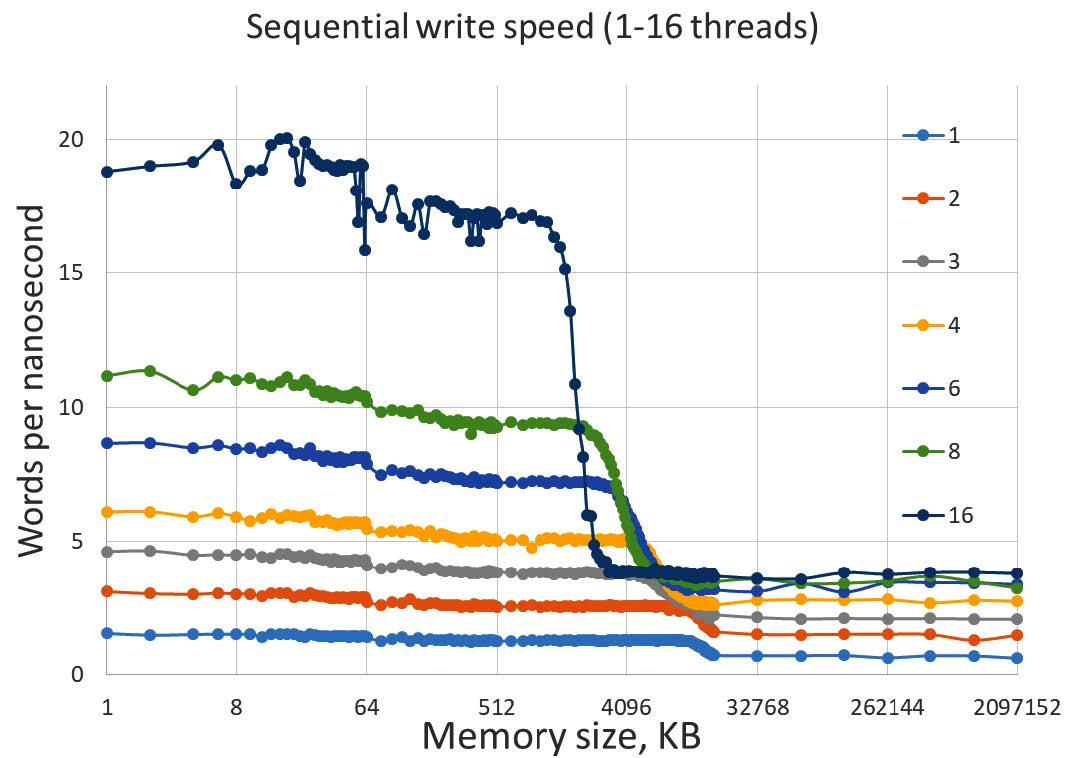
\includegraphics[width=0.9\textwidth]{content/1/chapter5/images/1.jpg}\\
Figure 5.1 – Memory throughput (words per nanosecond) for sequential writing of 64-bit integers as a function of memory range for 1 through 16 threads
\end{center}

The overall trend is already familiar to us: we see the speed jumps corresponding to the cache sizes. Now we focus on the differences between the curves for a different number of threads. We have the results for 1 through 16 threads (the machine used to collect these measurements does indeed have at least 16 physical CPU cores). Let us start from the left side of the plot. Here, the speed is limited by the L1 cache (up to 32 KB) then by the L2 cache (256 KB). This processor has separate L1 and L2 caches for each core, so, as long as the data fits into the L2 cache, there should not be any interaction between the threads since they don't share any resources: each thread has its own cache. In reality, this is not quite true, there are other CPU components that are still shared even for small memory ranges, but it's almost true: the throughput for 2 threads is twice as large as that for 1 thread, 4 threads write to memory twice as fast again, and 16 threads are almost 4 times faster than 4 threads.

The picture changes drastically as we exceed the size of the L2 cache and cross into the L3 cache and then the main memory: on this system, the L3 cache is shared between all the CPU cores. The main memory is shared too, although different memory banks are closer to different CPUs (the non-uniform memory architecture). For 1, 2, and even 4 threads, the throughput continues to scale with the number of threads: the main memory appears to have enough bandwidth for up to 4 processors writing into it at full speed. Then things take a turn for the worse: the throughput almost doesn't increase when we go from 6 to 16 threads. We have saturated the memory bus: it can't write the data any faster.

If this wasn't bad enough, consider that these results were obtained on the latest hardware at the time of writing (2020). In 2018, the same chart presented by the author in one of his classes looked like this:

\hspace*{\fill} \\ %插入空行
\begin{center}
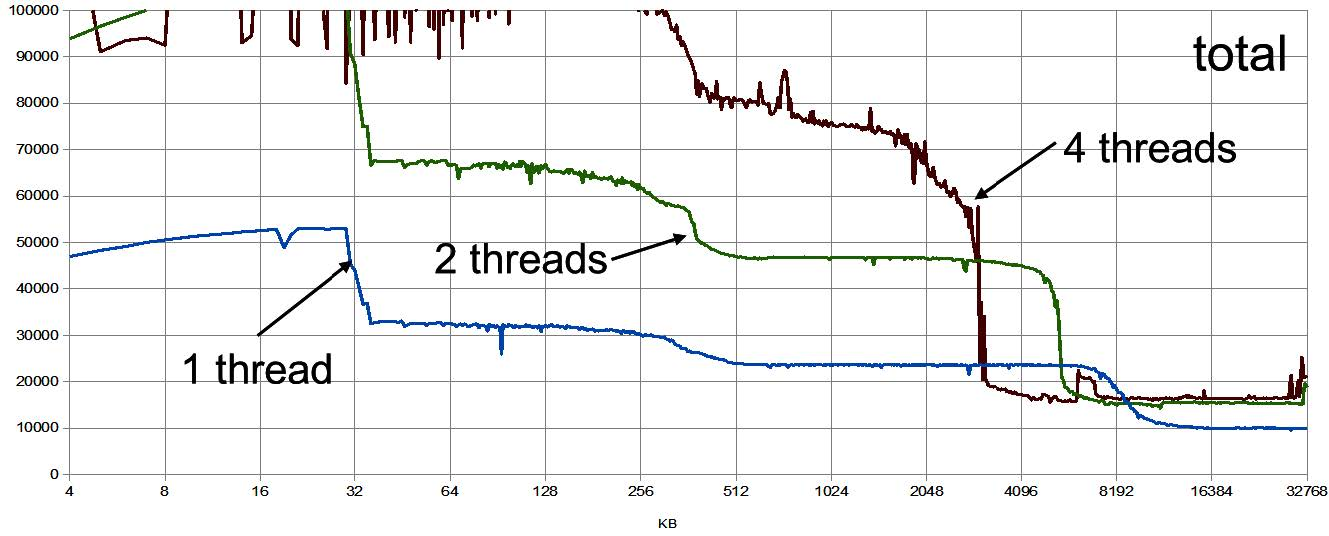
\includegraphics[width=0.9\textwidth]{content/1/chapter5/images/2.jpg}\\
Figure 5.2 – Memory throughput of an older (2018) CPU
\end{center}

This system has a memory bus that can be completely saturated by just two threads. Let us see what the implications of this fact for the performance of a concurrent program are.

\subsubsubsection{5.2.4\hspace{0.2cm}Memory-bound programs and concurrency}

The same results can be presented in a different way: by plotting the memory speed per thread versus the number of threads relative to that for one thread, we focus exclusively on the effect of concurrency on the memory speed:

\hspace*{\fill} \\ %插入空行
\begin{center}
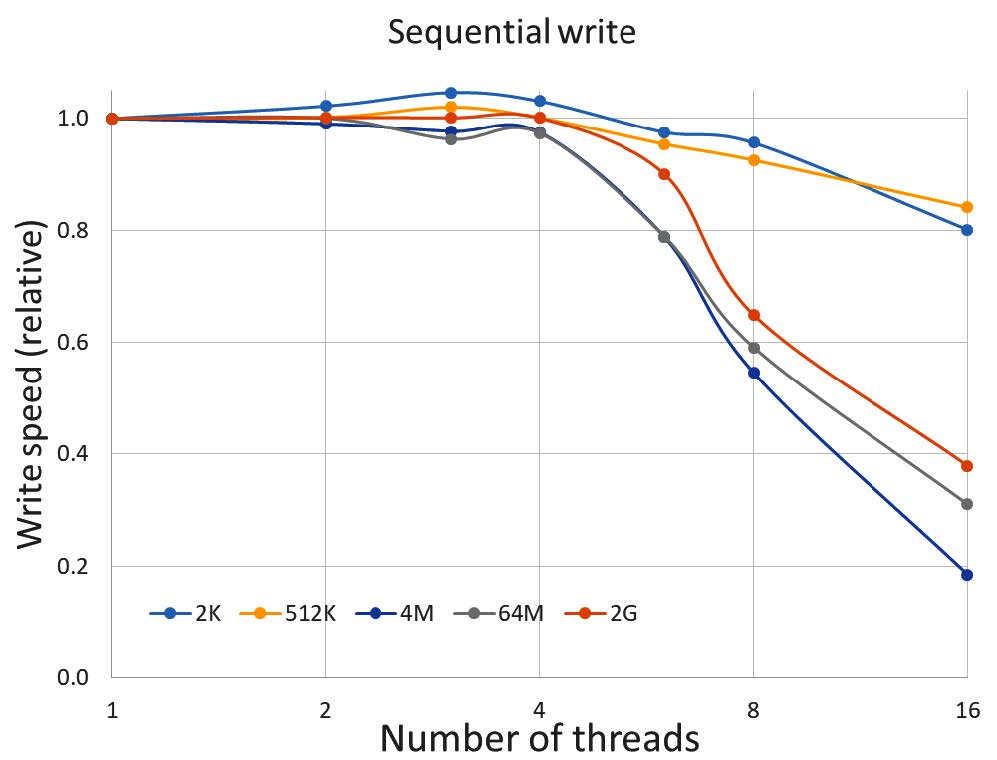
\includegraphics[width=0.9\textwidth]{content/1/chapter5/images/3.jpg}\\
Figure 5.3 – Memory throughput, relative to the throughput for a single thread, vs. thread count
\end{center}

With the memory speed normalized, so it's always 1 for the single thread, it is much easier to see that for small data sets that fit into L1 or L2 cache, the memory speed per thread remains almost the same even for 16 threads (each thread is writing at 80\% of its single-threaded speed). However, as soon as we cross into the L3 cache or exceed its size, the speed goes down after 4 threads. Going from 8 to 16 threads provides only minimal improvement. There just isn't enough bandwidth in the system to write data to memory fast enough. 

The results for different memory access patterns look similar, although the bandwidth for reading memory often scales slightly better than that for writing.

We can see that if our program was memory-bound in the single-threaded case, so its performance was limited by the speed of moving the data to and from the main memory, there is a fairly hard limit on the performance improvement we can expect to gain from concurrency. If you think that this does not apply to you because you don't have an expensive 16-core processor, remember that cheaper processors come with a cheaper memory bus, so most 4-core systems don't have enough memory bandwidth for all cores either.

For multi-threaded programs, it is even more important to avoid becoming memorybound. The implementation techniques that are useful here are splitting computations so more work can be done on smaller data sets that fit into L1 or L2 caches; rearranging the computations so more work can be done with fewer memory accesses, often at the expense of repeating some computations; optimizing the memory access patterns so the memory is accessed sequentially instead of randomly (even though you can saturate both access patterns, the total bandwidth of sequential accesses is much larger, so for the same amount of data your program may be memory-bound if you use random access and not limited by memory speed at all if you use sequential access). If the implementation techniques alone are insufficient and do not yield the desired performance improvements, the next step is to adapt the algorithm to the realities of concurrent programming: many problems have multiple algorithms that differ in their memory requirements. The fastest algorithm for a single-threaded program can often be outperformed by another algorithm that is better suited for concurrency: what we lose in the single-threaded execution speed, we make up for by brute force of scalable execution.

So far, we have assumed that each thread does its own work completely independently from all other threads. The only interaction between threads was indirect, due to contention for a limited resource such as memory bandwidth. This is the easiest kind of program to write, but most real-life programs do not allow such limitations. This brings with it a whole new set of performance problems, and it is time for us to learn about them.


















